\section{Class diagram}
A class diagram helps to create an understanding of the design of the system.
The following diagram illustrates the relevant classes related to the problem domain for the system.
It illustrates structural relations between classes and objects.

\begin{figure}[H]
    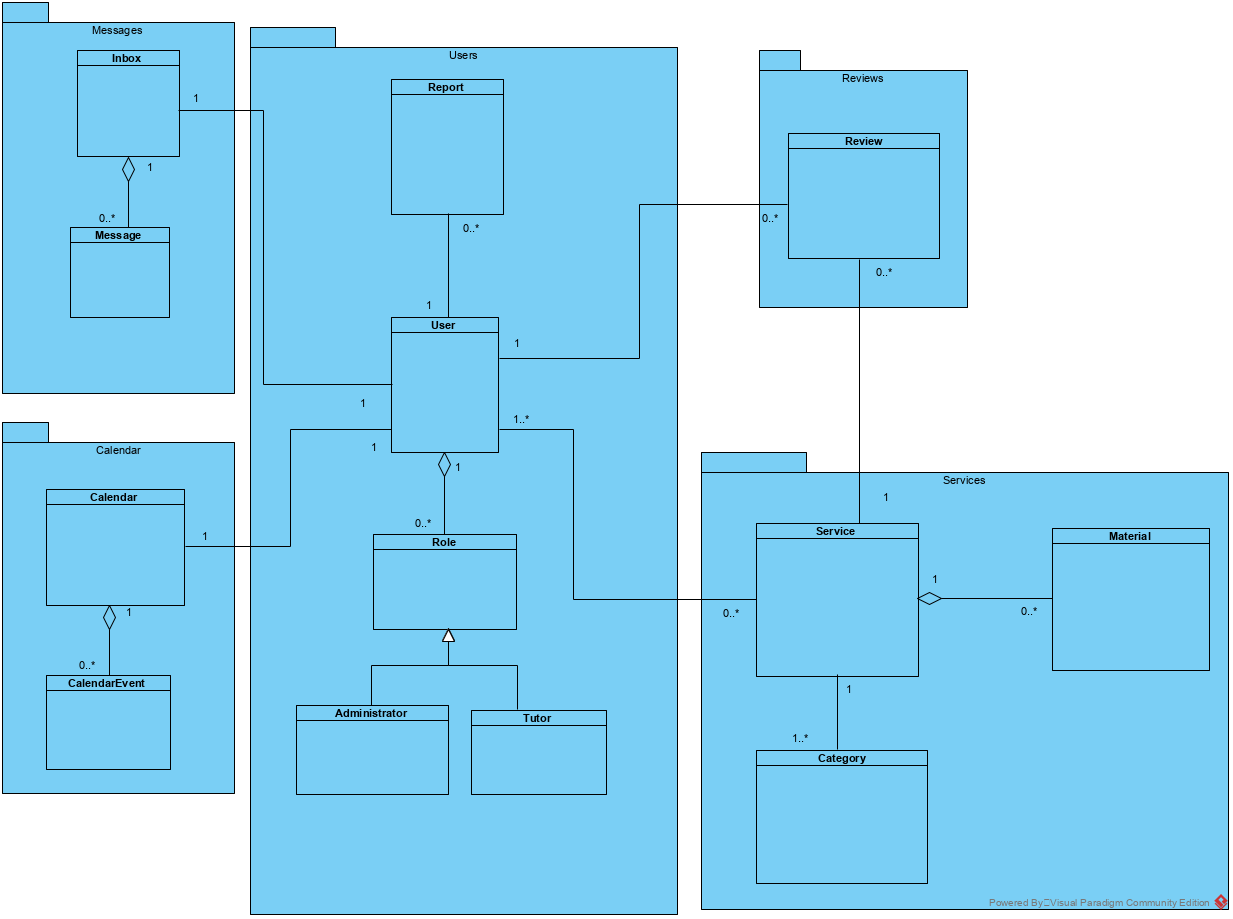
\includegraphics[width=\linewidth]{/tutorclassdiagram.png}
     \caption{The class diagram describing classes in the problem domain}
     \label{fig:class-diagram}
 \end{figure}

\subsection{Users}
Users are defined through the users cluster.
A user aggregates 0 or more roles. 
A role is a generalization of either the tutor or administrator classes. 
The role class ensures that the user can have both of the different roles, only one role or neither role, and that it can be dynamically changed.
If a user does not have a role, the user is simply regarded as a user of the system - a person seeking a tutor. 
Reports are used to ensure that the system is trustworthy and prevent the same problems recurring in interactions between students and tutors.
A tutor is associated with reports through an association relation.
A tutor will be associated with 0 or more reports, depending on how many times students have reported the tutor in question.
A tutor is also associated with 0 or more reviews in the same way. 
Students can rate their interactions with a tutor through the review.

\subsection{Calendar}
The calendar is the part of the system through which students and tutors establish dates on which to meet. 
One calendar is associated with one user.
A calendar aggregates 0 or more calendar events. 
The calendar does not need an event, it can simply show the overall view of the month.

\subsection{Services}
A service is what the tutors provide through the system. 
A user is associated with a service.
The user can be associated with 0 or more services, meaning that if the user is not a tutor they do not need to provide a service, and if they are a tutor they can provide more than one. 
The service itself is associated with one or more users, meaning that if the service exists, it is attributed to at least one tutor.
If the service only consists of material and is based around self studies, it could have multiple tutors authoring it, meaning it would be necessary to attribute the service to both.
A service aggregates 0 or more materials. 
The tutor can choose to provide material for their service, as long as it is relevant. 
However, a service could also simply be the tutor teaching the student in person, without material through the system.
A service is associated with one or more categories.
If a service is provided, it is based around a subject that defines its category.
However, the service might be related to more than just that one category.
The category assigned could be more specific to provide more information for the student, such as trigonometry rather than mathematics.
In such cases it would likely also be valuable to be able to assign multiple categories.
